\subsection{JSON Web Tokens}
In the RFC-7519\cite{rcf-jwt}, the \acrfull{jwt} is defined as:
\begin{quote}
    \textit{\acrfull{jwt} is a compact claims representation format intended for space constrained environments such as \acrshort{http} Authorization headers and URI query parameters.  \acrfull{jwt}s encode claims to be transmitted as a \acrshort{json} object that is used as the payload of a \acrfull{jws} structure or as the plaintext of a \acrfull{jwe} structure, enabling the claims to be digitally signed or integrity protected with a \acrfull{mac} and/or encrypted. \acrshort{jwt}s are always represented using the \acrshort{jws} Compact Serialization or the \acrshort{jwe} Compact Serialization.}
\end{quote}

Basically a \acrshort{jwt} is a \acrshort{json} that has three parts:
\begin{itemize}
    \item \textbf{Header}: provides important information about the token.
    \item \textbf{Payload}: it contains the actual information that will be transmitted to the application. The information is provided as key-value pairs. The keys are called claims.
    \item \textbf{Signature}: It is created using the Base64 encoding of the header and payload, as well as the specified signing or encryption method. The structure is defined by \acrfull{jws}.
\end{itemize}
Below (figure \ref{fig:jwt-ex}) we can see an example of signed and unsigned \acrshort{jwt}.
\begin{figure}[h]
    \centering
    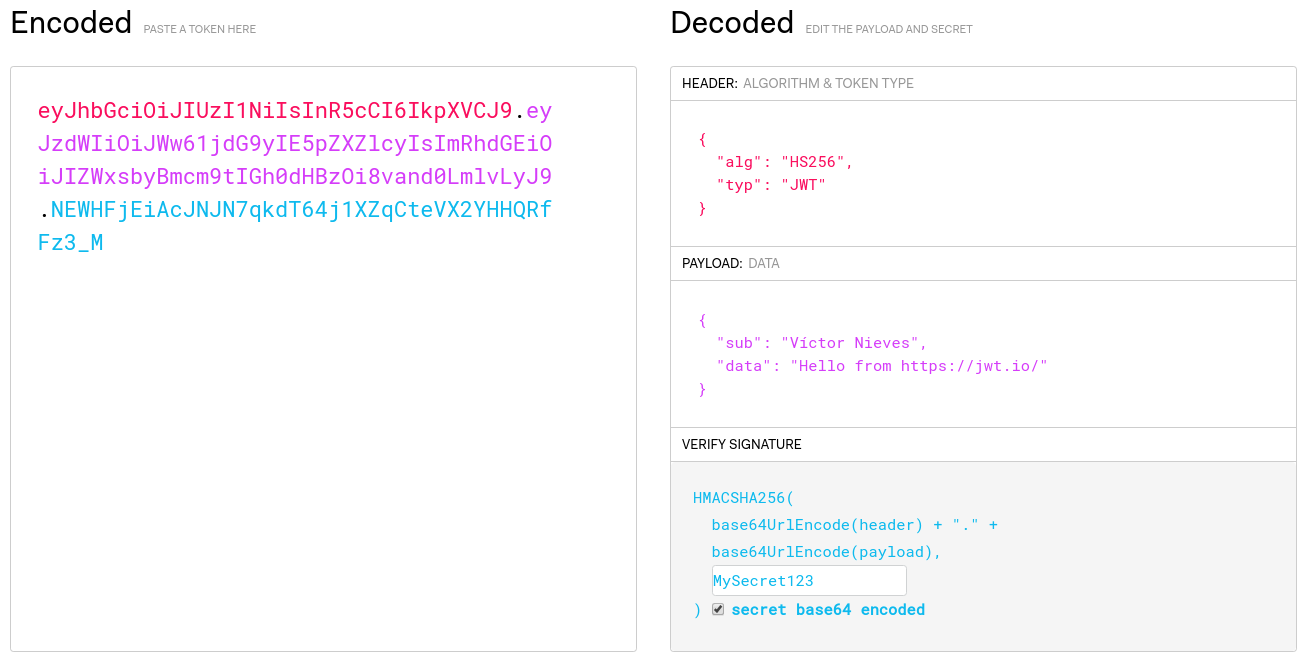
\includegraphics[width=1\textwidth]{images/State of the Art/jwts/jwt-example.png}
    \caption{Example of signed and unsigned \acrshort{jwt}}
    \label{fig:jwt-ex}
\end{figure}
